\documentclass{standalone}
\usepackage{tikz}
\usepackage{ctex,siunitx}
\setCJKmainfont{Noto Serif CJK SC}
\usepackage{tkz-euclide}
\usepackage{amsmath}
\usetikzlibrary{patterns, calc,3d}
\usetikzlibrary {decorations.pathmorphing,decorations.pathreplacing,decorations.shapes}
\tikzset{label style/.append style={font=\small}}
\begin{document}
\small
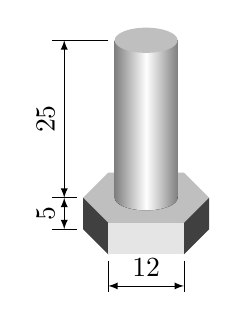
\begin{tikzpicture}[>=latex,scale=0.8]
  \fill[lightgray](-0.6,-0.4)--(0.6,-0.4)--(1,0)--(0.6,0.4)--(-0.6,0.4)--(-1,0)--cycle;
  \fill[darkgray](-1,0)--(-0.6,-0.4)--(-0.6,-0.9)--(-1,-0.5)--cycle;
  \fill[darkgray](1,0)--(0.6,-0.4)--(0.6,-0.9)--(1,-0.5)--cycle;
  \fill[lightgray!40](0.6,-0.4)rectangle(-0.6,-0.9);
  \fill[left color=gray,right color=gray,middle color=white](0,0)ellipse(0.5 and 0.2);
  \fill[left color=gray,right color=gray,middle color=white](-0.5,0)rectangle(0.5,2.5);
  \fill[lightgray](0,2.5)ellipse(0.5 and 0.2);
  \draw[very thin] (-0.6,-1)--(-0.6,-1.5)(0.6,-1)--(0.6,-1.5)(-1.1,0)--(-1.5,0)(-1.1,-0.5)--(-1.5,-0.5)(-0.6,2.5)--(-1.5,2.5);
  \draw[very thin,<->](-0.6,-1.4)--(0.6,-1.4)node[midway,above]{12};
  \draw[very thin,<->](-1.3,-0.5)--(-1.3,0)node[midway,sloped,above]{5};
  \draw[very thin,<->](-1.3,0)--(-1.3,2.5)node[midway,sloped,above]{25};
\end{tikzpicture}
\end{document}